\documentclass[11pt,a4paper]{article}
\usepackage[polish]{babel}
\usepackage[utf8]{inputenc}
\usepackage{polski}
\usepackage[T1]{fontenc}
\usepackage{ae,aecompl}
\frenchspacing
\usepackage[margin=2cm]{geometry}
\usepackage{graphicx}
\usepackage{float}
\usepackage{hyperref}
\usepackage{amsmath}
\usepackage{listings}
\usepackage{color}
\usepackage{epstopdf}
\lstset{
        basicstyle=\ttfamily,
        language=C,
        frame=single,
        keywordstyle=\color[rgb]{0,0,1},
        commentstyle=\color[rgb]{0.133,0.545,0.133},
        stringstyle=\color[rgb]{0.627,0.126,0.941},
        columns=flexible,
}

\begin{document}
\title{\LARGE  Projekt nr 2 \\ \vspace{0.4cm} \textbf{Monte Carlo - rozkład temperatury w 2-D}\\ w technologii Java RMI}
\author{Michał Drobniak, 
 Marcin Piłat }
\date{Maj 2013}
\maketitle

\vfill
\begin{figure}[H]
\begin{center}

\includegraphics[width=0.7\textwidth]{agh_nzw_s_pl_1w_wbr_rgb_150ppi.jpg}
\end{center}
\end{figure}
\newpage

\section{Wstęp}

Program służy do obliczania temperatury na płytce dwuwymiarowej w oparciu o znaną temperaturę na brzegach za pomocą metody Monte Carlo. Płytka dzielona jest na siatkę N na N.\\
Rozkład temperatury wewnątrz jest opisana przez równanie Laplace'a, tzn. że temp. w każdym punkcie jest średnią temp. punktów otaczających go (z góry, prawej, dołu i lewej).\\
\\
Metoda \textbf{Monte Carlo} używana jest do wyznaczenia temp. w danym punkcie S, poprzez:
\begin{enumerate}
	\item Losowe wybranie jednego z 4 sąsiadów
	\item Dodawanie jego temperatury do sumy
	\item Przeprowadzenie powyższych operacji n razy
	\item Podzielenie sumy przez n
\end{enumerate}
Wynikiem końcowym jest przybliżona \textbf{temperatura w punkcie S}.\\
\\
Ponieważ nie znane są temp. sąsiadów, więc używając tej samej metody można wyznaczyć ich temperatury rekursywnie, poprzez \textbf{losowe przechodzenie} po płytce. Rekursja skończy się, ponieważ napotka jedną z krawędzi na której temp. jest znana.

\begin{figure}[H]
\begin{center}
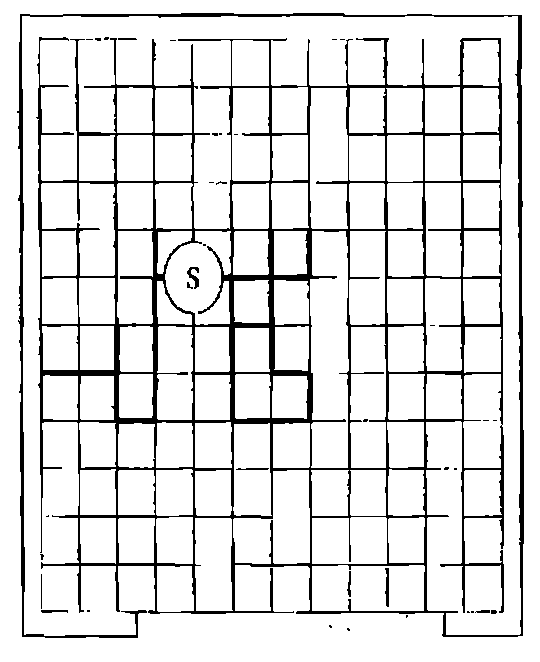
\includegraphics[width=0.4\textwidth]{random_walk.png}
\caption{Schemat losowego przechodzenia po płytce}
\end{center}
\end{figure}

\section{Opis implementacji algorytmu}
Powyższy algorytm został zaimplementowany z jedną różnicą: na potrzeby wielowątkowości każdy proces oblicza 500 próbek temperatur (niezależnie od tego, czy się zbiegają, czy nie) i następnie oblicza temperaturę dzieląc ją przez liczbę próbek.\\
\\
Zgodnie z zasadami technologi Java RMI, implementacja tego algorytmu znajduje się w kodzie po stronie serwera, w odpowiedniej klasie implementującej publiczny interfejs (Api). Dzięki wiedzy że obiekt namiastki na pewno implementuje w powyższy sposób algorytm liczący temperaturę, można swobodnie zażądać wykonania metody temperature() na tym obiekcie po stronie klienta. Metoda ta zwróci wyliczoną temperaturę w zadanym punkcie [x,y] na podstawie aktualnej siatki p[N][N]. Każde żądanie uruchamiane jest jako nowy wątek przesłany do kolejnych serwerów, więc to klient odpowiedzialny jest za samą wielowątkowość.
\\
Obliczone i początkowe temperatury przechowujemy w tablicy o wymiarach N na N. Wszystkie temperatury oprócz brzegowych są zainicjalizowane wartością -1 (można tak zrobić, ponieważ Kelwiny nie przyjmują ujemnych wartości). Brzegowe temperatury są inicjalizowane zgodnie z treścią zadania: trzy ściany $0^{\circ}$ i czwarta $100^{\circ}$. Dlatego znana temperatura to temperatura większa lub równa $0^{\circ}$.

\begin{figure}[H]
\begin{center}
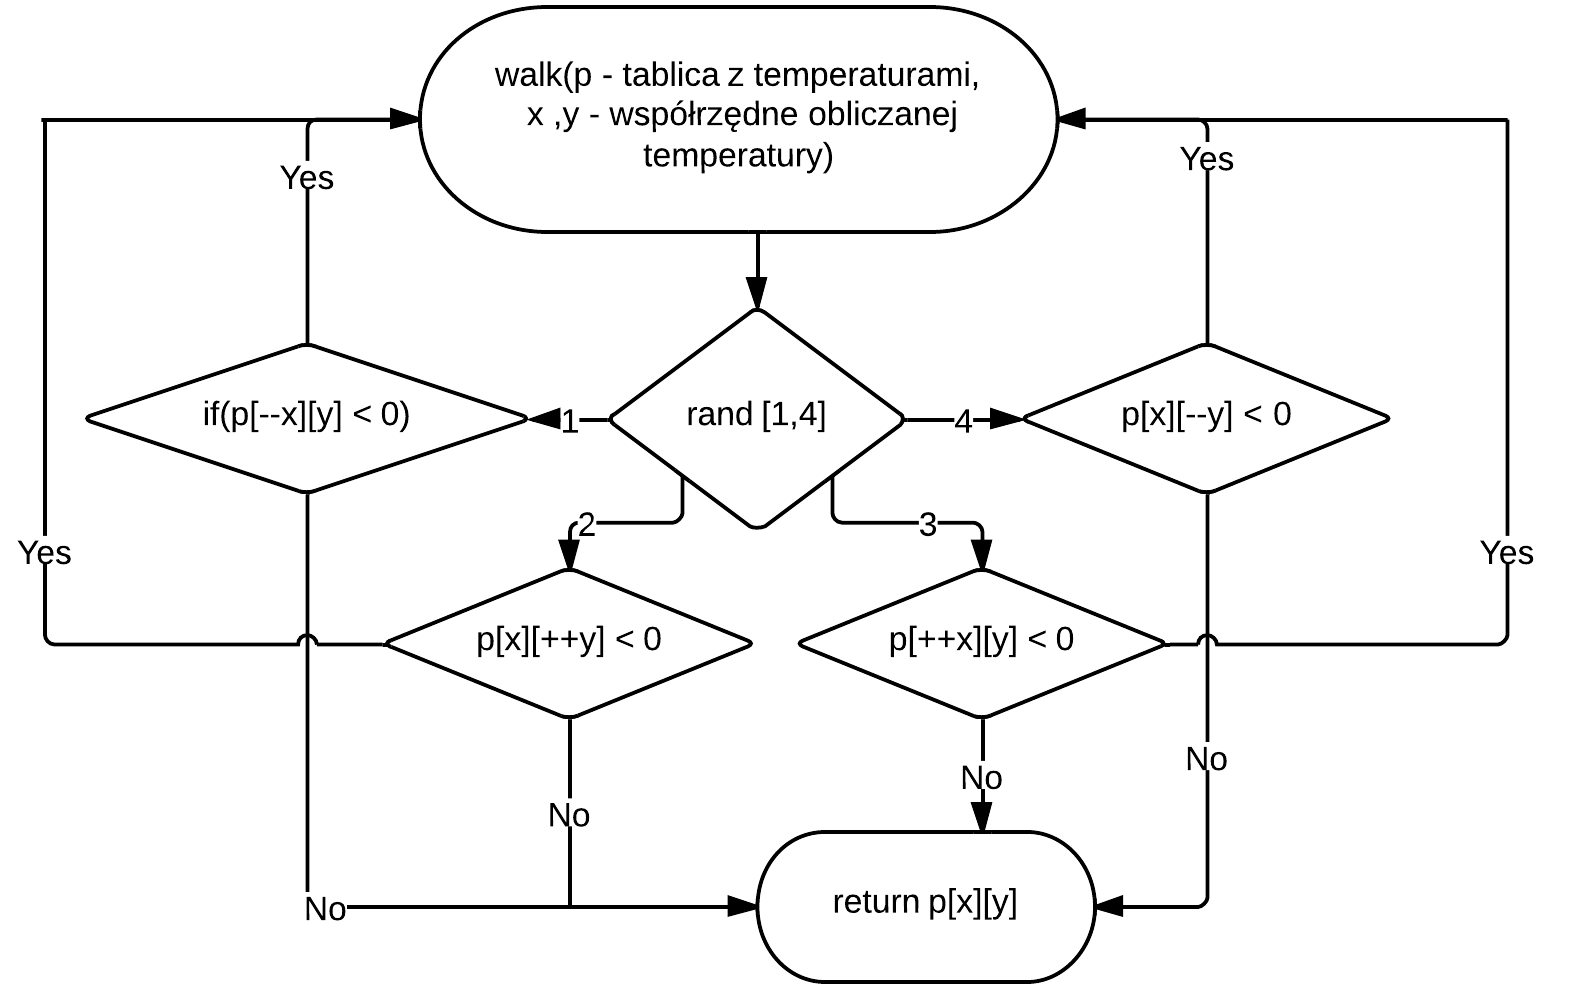
\includegraphics[width=0.7\textwidth]{schemat2.png}
\caption{Schemat blokowy poszukiwania znanej temperatury}
\end{center}
\end{figure}

\begin{figure}[H]
\begin{center}
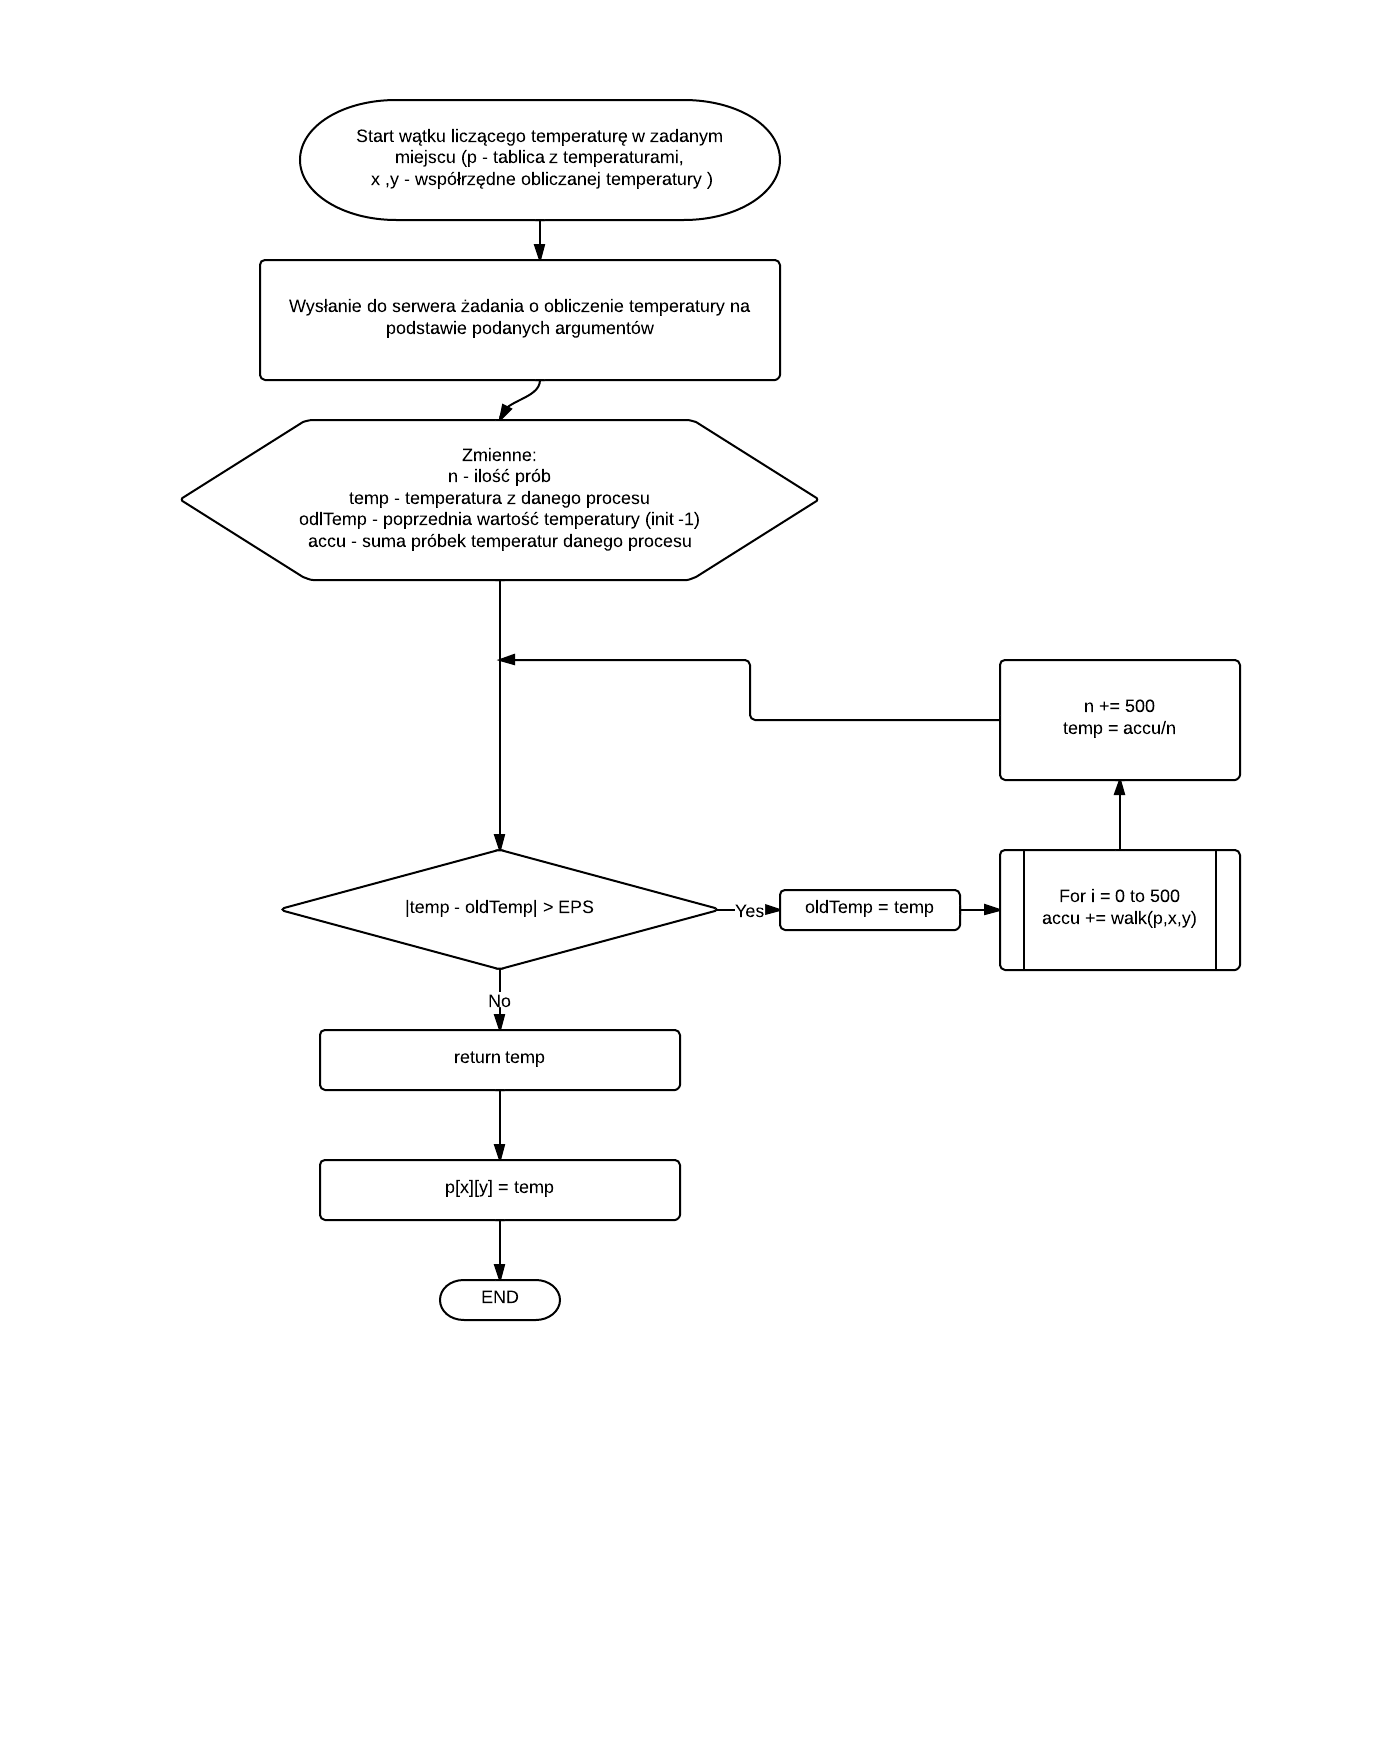
\includegraphics[width=1.0\textwidth]{schemat1.png}
\caption{Schemat blokowy obliczania temperatury w punkcie danym współrzędnymi x i y}
\end{center}
\end{figure}





\section{Prezentacja i interpretacja wyników}

Płytka została zainicjalizowana w następujący sposób:
\begin{enumerate}
	\item Krawędzie dolna, lewa, górna mają temperaturę $0^{\circ}$
	\item Krawędź prawa ma temperaturę $100^{\circ}$
\end{enumerate}

\begin{figure}[H]
\begin{center}
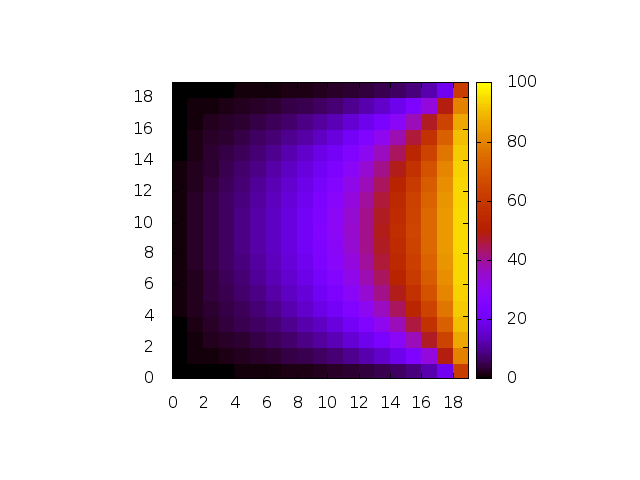
\includegraphics[width=0.7\textwidth]{grid.png}
%\includegraphics[width=0.7\textwidth,angle=-90]{grid.eps}
\caption{Wykres płytki w gnuplocie}
\end{center}
\end{figure}

Jak widać na powyższym wykresie płaszczyzny, najwyższa temp. jest przy prawej krawędzi, stopniowo malejąc w kierunku przeciwnym, w dół oraz w górę, co jest zgodne z oczekiwanym rozkładem temperatury na płytce.

Dodaliśmy również wizualizację rozkładu ciepła na płytce w programie. W tym celu korzystaliśmy z klasy rysującej mapę ciepła napisanej przez Matthew Beckler, Josh Hayes-Sheen i J. Keller. Klasa ta jest udostępniana na licencji GNU. 

\begin{figure}[H]
\begin{center}
\includegraphics[width=0.5\textwidth]{heatMapProg.png}
\caption{Wykres płytki w programie}
\end{center}
\end{figure}

\section{Opis uruchamiania programu}

Kompilację i uruchomienie programu, można przeprowadzić używając dostarczonego wraz z programem pliku \textbf{Makefile}.\\
Do kompilacji można wykorzystać polecenia:
\begin{enumerate}
	\item \textbf{'make all'} - kompilacja wszystkich klas z pakietów Api, Client i Server
\end{enumerate}
Do uruchomienia można wykorzystać polecenia:
\begin{enumerate}
	\item \textbf{'run\_server'} - uruchomienie 2 serwerów na kolejnych portach
	\item \textbf{'run\_client'} - uruchomienie klienta korzystającego z 2 uprzednio uruchomionych serwerów
\end{enumerate}

\end{document}
